\documentclass[12pt]{article}
\usepackage{scrtime} % for \thistime (this package MUST be listed first!)
\usepackage[margin=1in]{geometry}
\usepackage{subfig}

%% Language and font encodings
\usepackage[english]{babel}
\usepackage[utf8x]{inputenc}
\usepackage[T1]{fontenc}

%% Useful packages
\usepackage{amsmath}
\usepackage{amsthm} % for theorems and proofs
\usepackage{amsfonts} % mathbb
\usepackage{graphicx}
\usepackage[colorinlistoftodos]{todonotes}
\definecolor{aqua}{RGB}{0, 128, 225}
\usepackage[colorlinks=true,citecolor=aqua,linkcolor=aqua,urlcolor=aqua]{hyperref}
\usepackage[nameinlink]{cleveref}

\usepackage{fancyhdr,lastpage}
\pagestyle{fancy}
\fancyhf{} % clear all header and footer parameters
%%%\lhead{Student Name: \theblank{4cm}}
%%%\chead{}
%%%\rhead{Student Number: \theblank{3cm}}
%%%\lfoot{\small\bfseries\ifnum\thepage<\pageref{LastPage}{CONTINUED\\on next page}\else{LAST PAGE}\fi}
\lfoot{}
\cfoot{{\small\bfseries Page \thepage\ of \pageref{LastPage}}}
\rfoot{}
\renewcommand\headrulewidth{0pt} % Removes funny header line

\newcommand{\R}{{\cal R}}

\title{Math 4MB3: Draft Group Project}
\author{\underline{\emph{Group Name}}: \texttt{{\color{blue}The Infective Collective}}\\
{}\\
\underline{\emph{Group Members}}: {\color{blue}Aurora Basinski-Ferris, Michael Chong, Daniel Park, Daniel Presta}}

\date{\today\ @ \thistime}



\begin{document}
\maketitle

\section{Introduction}
(Daniel Presta, Michael)

\begin{itemize}
\item synchrony
\item implications
\item context and motivation
\item outline of the rest of the things
\end{itemize}

In epidemiological systems, spatial synchrony and coherence within populations are of immense importance. Determining the conditions under which an epidemiological model becomes coherent aids in the eradication of pathogens \cite{earn1998persistence}. Epidemiologists wish to create a synchronous system in which the extinction of parasites occurs in all patches simultaneously, for this will prevent against any ``rescue effects'' \cite{Earn2000conservation}. Once this extinction occurs, we will have totally eliminated the existence and possible transmission of the disease.

The rest of this paper is structured as follows. In \Cref{sec:construction} we show the construction of the discrete time SIR model we will investigate in this paper. In \Cref{sec:numerical} we describe our numerical simulation setup, and explore the parameter space with respect to synchrony. We end with a discussion in \Cref{sec:discussion} where we compare our findings for this model to continuous time SIR models and connect our results to implications for infectious disease control.

(remove analytical, different seasonal forcing, focus on discussing stochasticity, exploring parameter space, mixing structure) 

\section{Methods}

\subsection{Mathematical model}
\label{sec:construction}

In this study, we use an SIR (Susceptible-Infected-Recovered) model with time dependent transmission rate.
As it is challenging to implement demographic stochasticity in a coupled ODE system and computationally exhaustive to solve such system, we use a discrete time model for convenience.
The model is constructed based on an ODE model by interpreting the rate at which individuals leave their compartments as hazards (See supplementary file for full details).
For simplicity, we ignore exposed period as it does not have much effect on the qualitative dynamics of the system.

Consider $n$ patches of populations connected with each other.
Let $S_k(t), I_k(t), R_k(t)$ denote number of susceptible, infected, and recovered individuals in patch $k$ at time $t$.
Assuming that the individuals do not immigrate to other patches but simply contact individuals in other patches for a short period of time, the discrete-time SIR model is given by
\begin{equation}
\label{eq:discretedeterministic}
\begin{aligned}
S_{k}(t+\Delta t) &= b_k(t) + S_k(t) - S_{k, \tiny{\textrm{leave}}}(t)\\
I_{k}(t+\Delta t) &= i_k(t) + I_k(t) - I_{k, \tiny{\textrm{leave}}}(t)\\
R_{k}(t+\Delta t) &= r_k(t) + R_k(t) - R_{k, \tiny{\textrm{leave}}}(t)
\end{aligned}
\end{equation}
where $S_{k, \tiny{\textrm{leave}}}(t)$, $I_{k, \tiny{\textrm{leave}}}(t)$, and $R_{k, \tiny{\textrm{leave}}}(t)$ are number of susceptible, infected, and recovered individuals in patch $k$ that leave their compartments between time $(t, t + \Delta t)$, respectively, and $b_k(t)$, $i_k(t)$ and $r_k(t)$ represent number of new susceptible, infected, and recovered individuals that are produced between time interval $(t, t+\Delta t)$:
\begin{equation}
\begin{aligned}
S_{k, \tiny{\textrm{leave}}}(t) &= \left(1 - \exp \left(-\left(\sum_{j=1}^n \beta(t) m_{ij} I_j(s) + \mu \right) \Delta t \right) \right) S_i(t)\\
I_{i, \tiny{\textrm{leave}}}(t) &= (1 - \exp(-(\gamma + \mu)\Delta t)) I_i(t) \\
R_{i, \tiny{\textrm{leave}}}(t) &= (1 - \exp(-\mu \Delta t)) R_i(t) \\
i_k(t) &= \frac{\sum_{j=1}^n \beta(t) m_{kj} I_j(s)}{\sum_{j=1}^n \beta(t) m_{kj} I_j(s) + \mu} S_{k, \tiny{\textrm{leave}}}(t)\\
r_k(t) &= \frac{\gamma}{\gamma + \mu} R_{k, \tiny{\textrm{leave}}}(t)\\
b_k(t) &= S_{k, \tiny{\textrm{leave}}}(t) - i_k(t) + I_{k, \tiny{\textrm{leave}}}(t) - r_k(t)\\
\end{aligned}
\end{equation}
where $\beta(t)$ is the transmission rate, $m_{kj}$ is the proportion of contact dispersed to patch $k$ from patch $j$, $\gamma$ is the per capita recovery rate, and $\mu$ is the per capita natural death rate. 
Note that by defining natural birth ($b_k(t)$) in a such way, we are keeping population size identically constant in every patch.

Since this model is constructed based on a probabilistic argument, adding demographic stochasticity model simply requires adding appropriate binomial random variables based on the derived probabilities. Then, the model structure remains the same but instead we have
\begin{equation}
\begin{aligned}
S_{k, \tiny{\textrm{leave}}}(t) &= \mathrm{Binom}\left(S_k(t), 1 - \exp \left(-\left(\sum_{j=1}^n \beta(t) m_{ij} I_j(s) + \mu \right) \Delta t \right)\right)\\
I_{k, \tiny{\textrm{leave}}}(t) &= \mathrm{Binom}\left(I_k(t), 1 - \exp \left(-\left(\gamma + \mu \right) \Delta t \right)\right)\\
R_{k, \tiny{\textrm{leave}}}(t) &= \mathrm{Binom}\left(R_k(t), 1 - \exp \left(-\mu \Delta t \right)\right)\\
i_k(t) &= \mathrm{Binom}\left(S_{k, \tiny{\textrm{leave}}}(t), \frac{\sum_{j=1}^n \beta(t) m_{ij} I_j(s)}{\sum_{j=1}^n \beta(t) m_{ij} I_j(s) + \mu}\right)\\
r_k(t) &= \mathrm{Binom}\left(R_{k, \tiny{\textrm{leave}}}(t), \frac{\gamma}{\gamma + \mu}\right) \\
b_k(t) &= S_{k, \tiny{\textrm{leave}}}(t) - i_k(t) + I_{k, \tiny{\textrm{leave}}}(t) - r_k(t)\\
\end{aligned}
\end{equation}

\subsection{Time dependent transmission rate}

In order to generate interesting results, we express the transmission rate $\beta (t)$ as a time-dependent function. Our first approach was to employ sinusoidal forcing of the contact rate, a method explored in \cite{aron1984seasonality} and \cite{olsen1990chaos}. From \cite{keeling2002understanding}, we observe the sinusoidally forced, time-dependent transmission rate, given by
\begin{equation}
\begin{aligned}
\beta (t) &= b_0  (1 + b_1 \sin (2\pi t)),
\end{aligned}
\end{equation}
where $b_0$ represents the mean transmission rate, and $b_1$ represents the amplitude of seasonal forcing.
After observing the results displayed in \autoref{fig:seasamp}, we consider a more complex model of the transmission rate. Since transmission rates depend highly on the contact rates between children \cite{keeling2002understanding}, it appears sensible to express $\beta (t)$ as a step function. Assuming that $\beta (t)$ is expressed differently during the school months than during the holidays (and that it respects those trends) \cite{he2009plug}, we observe the term-time forced, time-dependent transmission rate, posed in \cite{bauch2003interepidemic}:
\begin{equation}
\begin{aligned}
\beta (t) &= 
\begin{cases} b_0 (1 + 2(1 - p_s) b_1) &\mbox{school days} \\ 
b_0 (1 - 2 p_s b_1) & \mbox{non-school days}
\end{cases}.
\end{aligned}
\end{equation}
In this function, the definitions of $b_0$ and $b_1$ remain the same, while $p_s = 0.7589$ represents the estimated proportion of the year taken up by the school terms. The results when coherence is measured with term-time forcing of the transmission rate is displayed in \autoref{fig:seasamp}.

\subsection{Parameters of the model}

Unless otherwise stated, we use parameters that give rise to similar qualitative dynamics as measles throughout this paper. In particular, we use $\R_0 = 17$, $\gamma = 365/13 \text{years}^{-1}$, $N = 1,000,000$, $\mu = 0.02 \text{years}^{-1}$, $\Delta t = 1/365 \text{years}$ as our baseline parameters \cite{earn2000simple} unless specified otherwise. To account for the lack of exposed period, we let length of infectious period to be the sum of exposed and infectious periods of measles. 

Previous studies have shown that seasonally forced models can give rise to complex dynamics ranging from periodic cycles to chaos [CITE]. We are focusing on these parameters specifically in this draft as it can lead to incoherent dynamics 

\subsection{Numerical analysis}
This paper utilizes numerical methods to investigate the behaviour of the model constructed in \Cref{sec:construction}. Thus, we first implemented the deterministic model given in \autoref{eq:discretedeterministic} in R. We initialized the parameters in R, but implemented the rest of the model using the \texttt{Rcpp} package due to the faster speeds of \texttt{C++} when utilizing nested \texttt{for} loops. The results of the model (number of individuals infected, susceptible, and recovered in each patch) were stored in a dataframe and passed back to R to be analyzed.

The numerical investigations were focused on categorizing the synchronous behaviour of the model when modifying various parameters. The investigations of the deterministic model fell into the categories of: modifying the seasonal forcing, modifying the mixing structure, and changing $\R_0$ (the results for these modifications can be found in \Cref{ss:seasonalforcing}, \Cref{ss:mixingstructure}, and \Cref{ss:parameters} respectively). Finally, we added stochasticity by adding binomial random variables (described in \Cref{sec:construction}) and compared the synchronous behaviour of the model to the deterministic case with similar parameter choices.

\section{Results} \label{sec:numerical}
\subsection{Seasonal Forcing}
\label{ss:seasonalforcing}

We begin by exploring the effects of the two seasonal forcing functions on coherence. For both the sinusoidally forced transmission rate and the term-time forced transmission rate, different values for the seasonal amplitude $b_1$ were tested to see if coherence (or the degree of coherence) was affected in any way. In all simulations, the connectivity matrix
$$
\begin{bmatrix}
0.999 & 0.001\\
0.001 & 0.999
\end{bmatrix}
$$
was used.

\begin{figure}
\centering
\subfloat{(a)}
{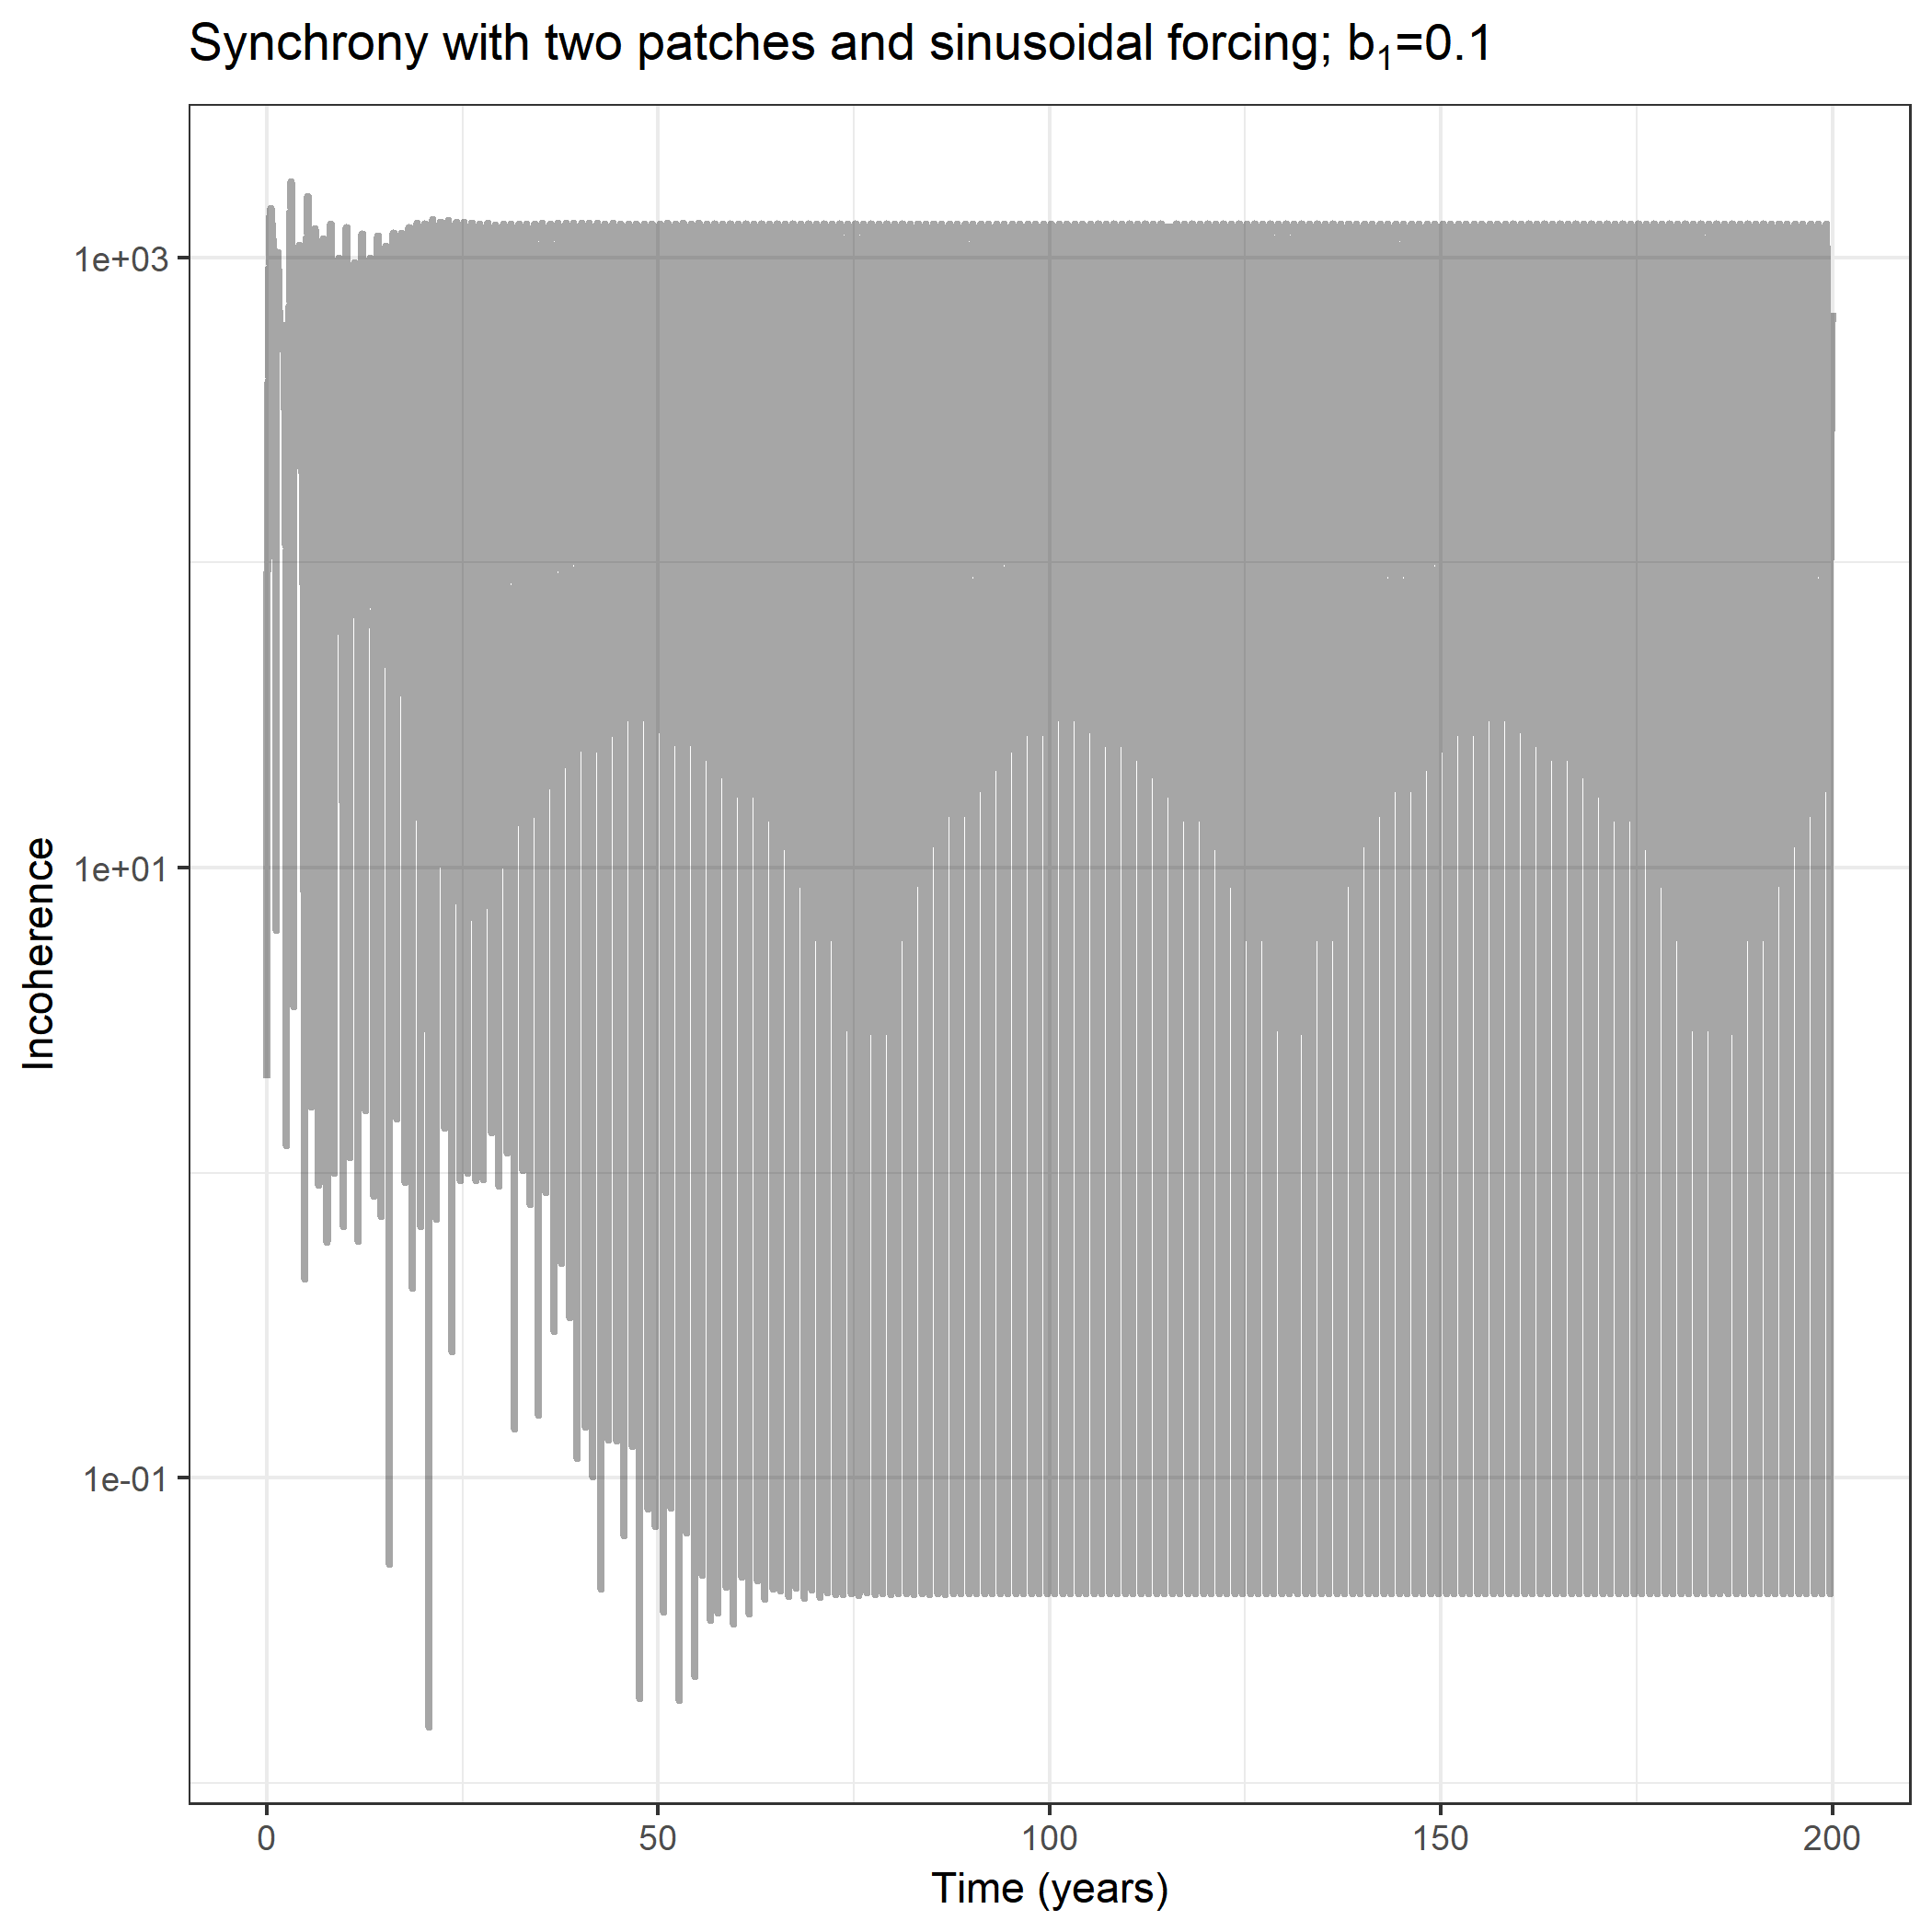
\includegraphics[width=.4\linewidth]{seasonalamp_1.png}} \quad
\subfloat{(b)}
{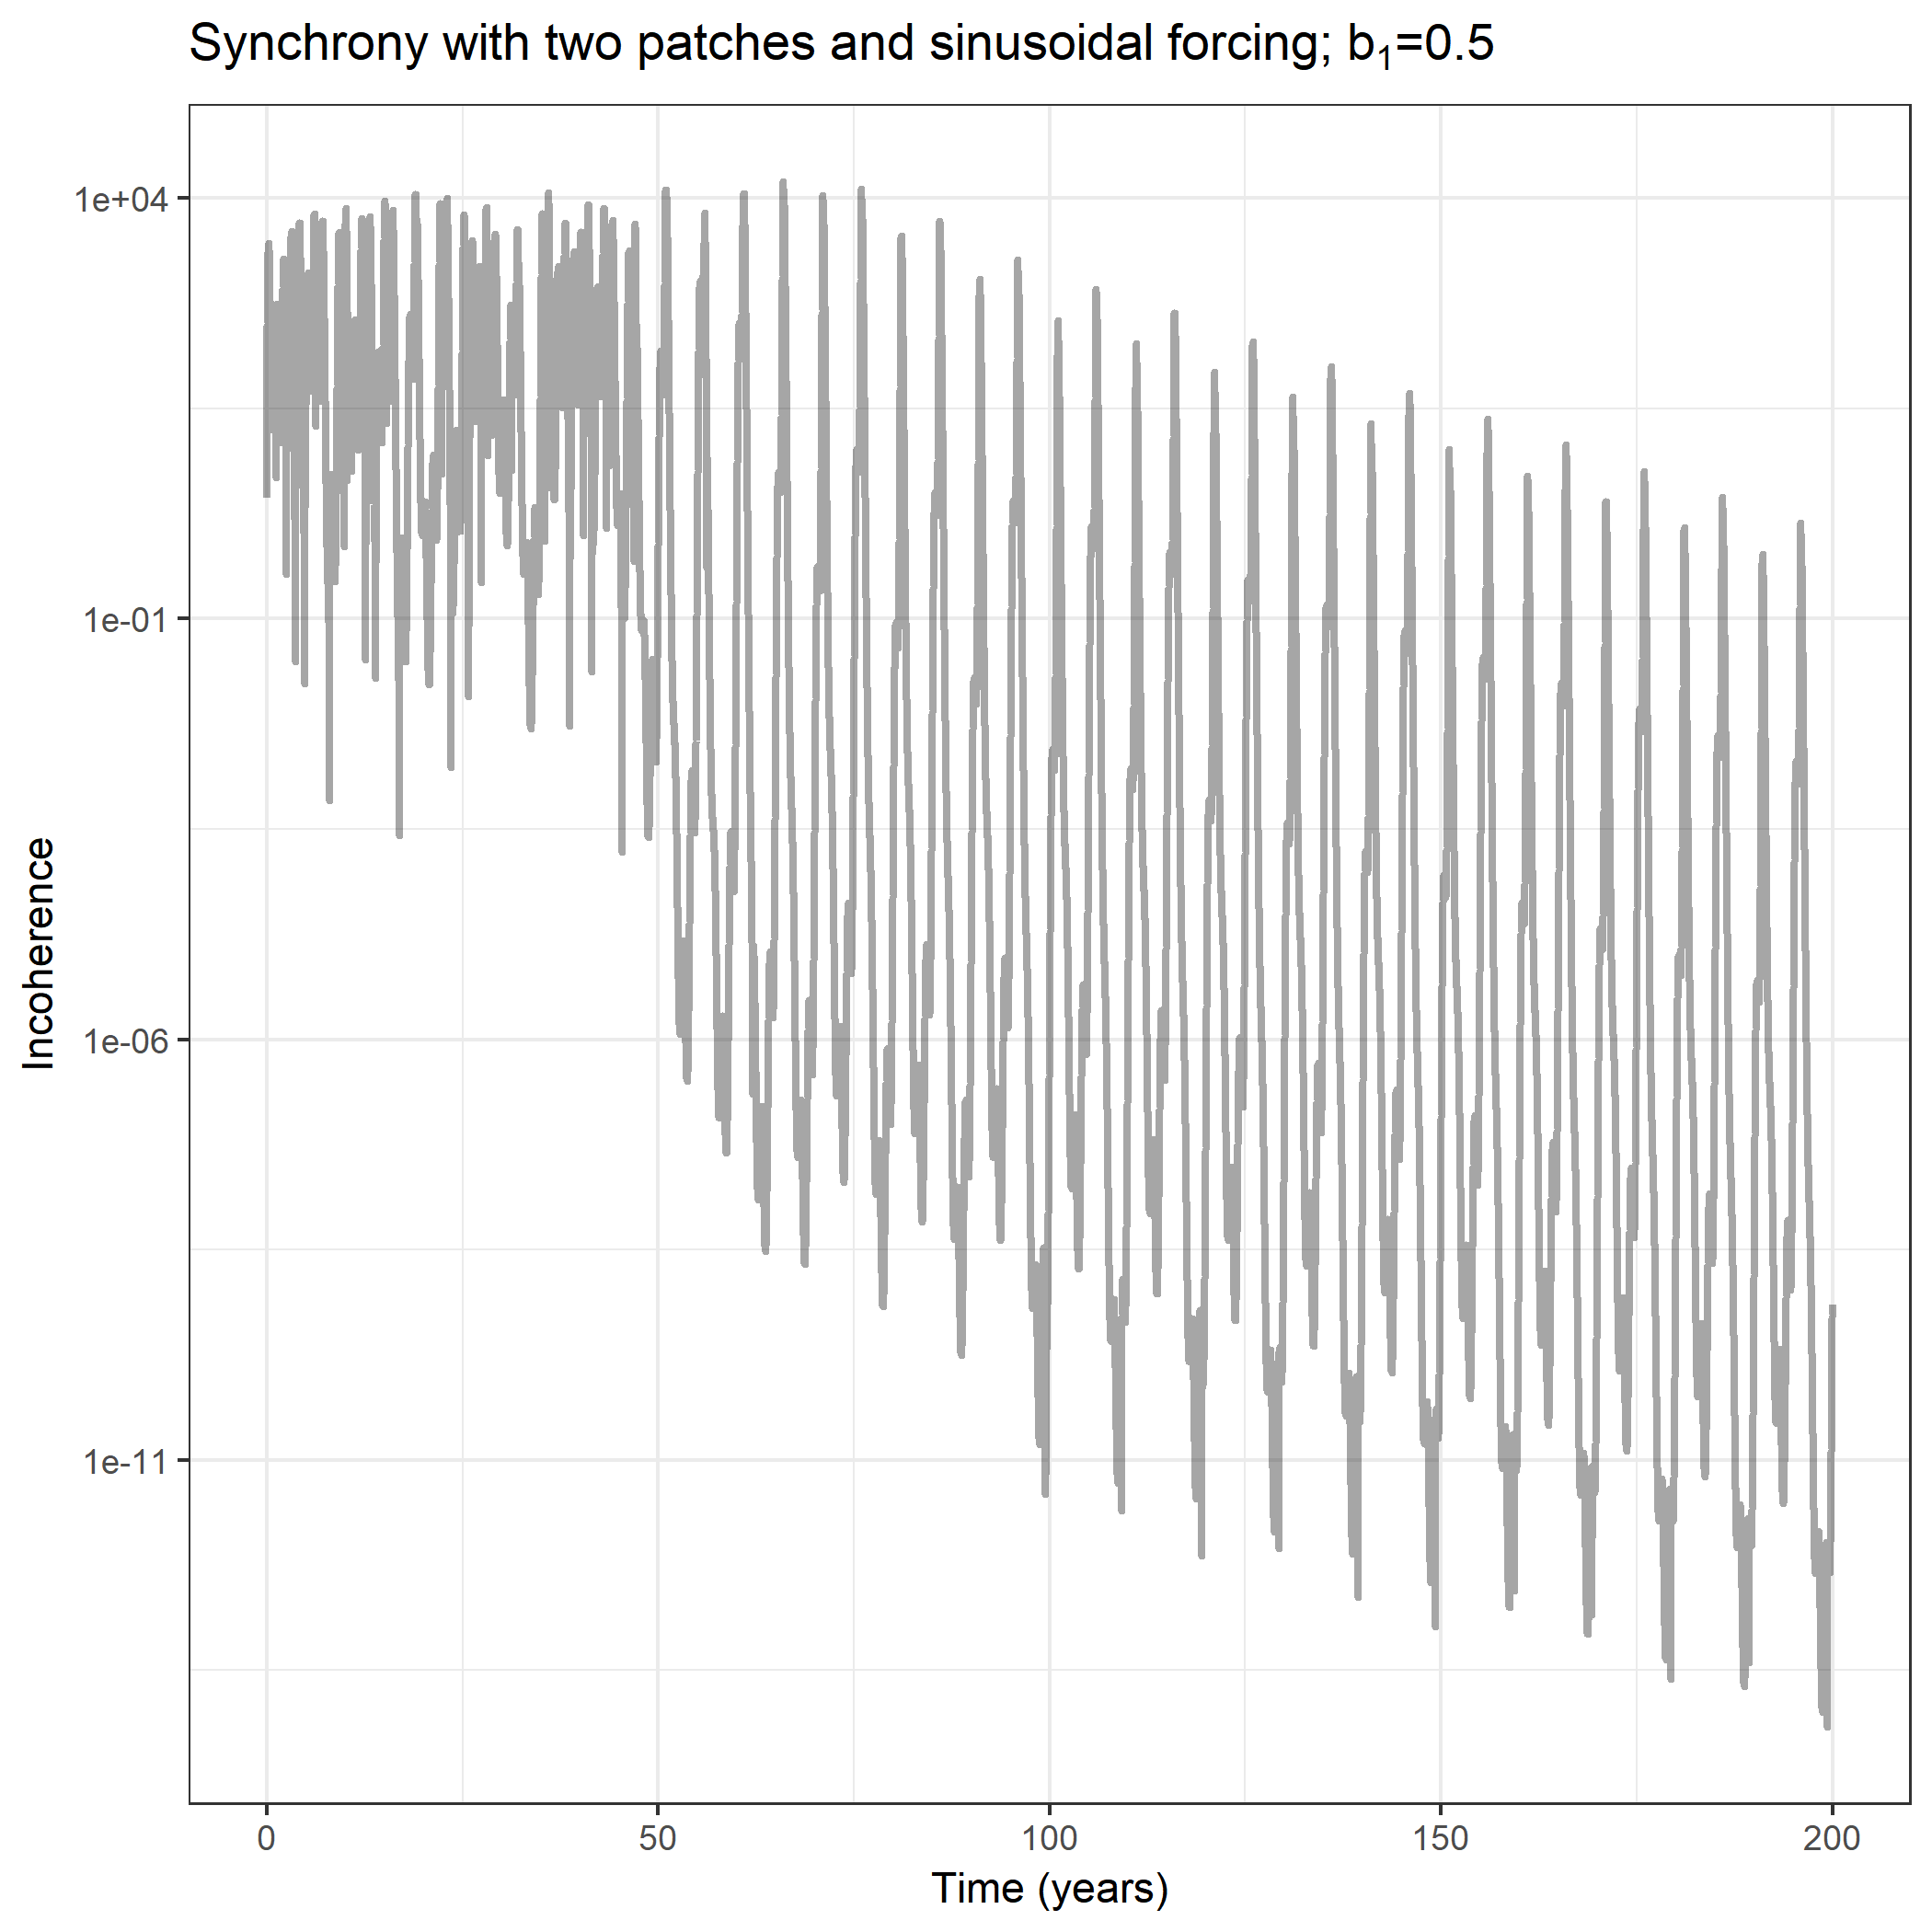
\includegraphics[width=.4\linewidth]{seasonalamp_2.png}} \\
\subfloat{(c)}
{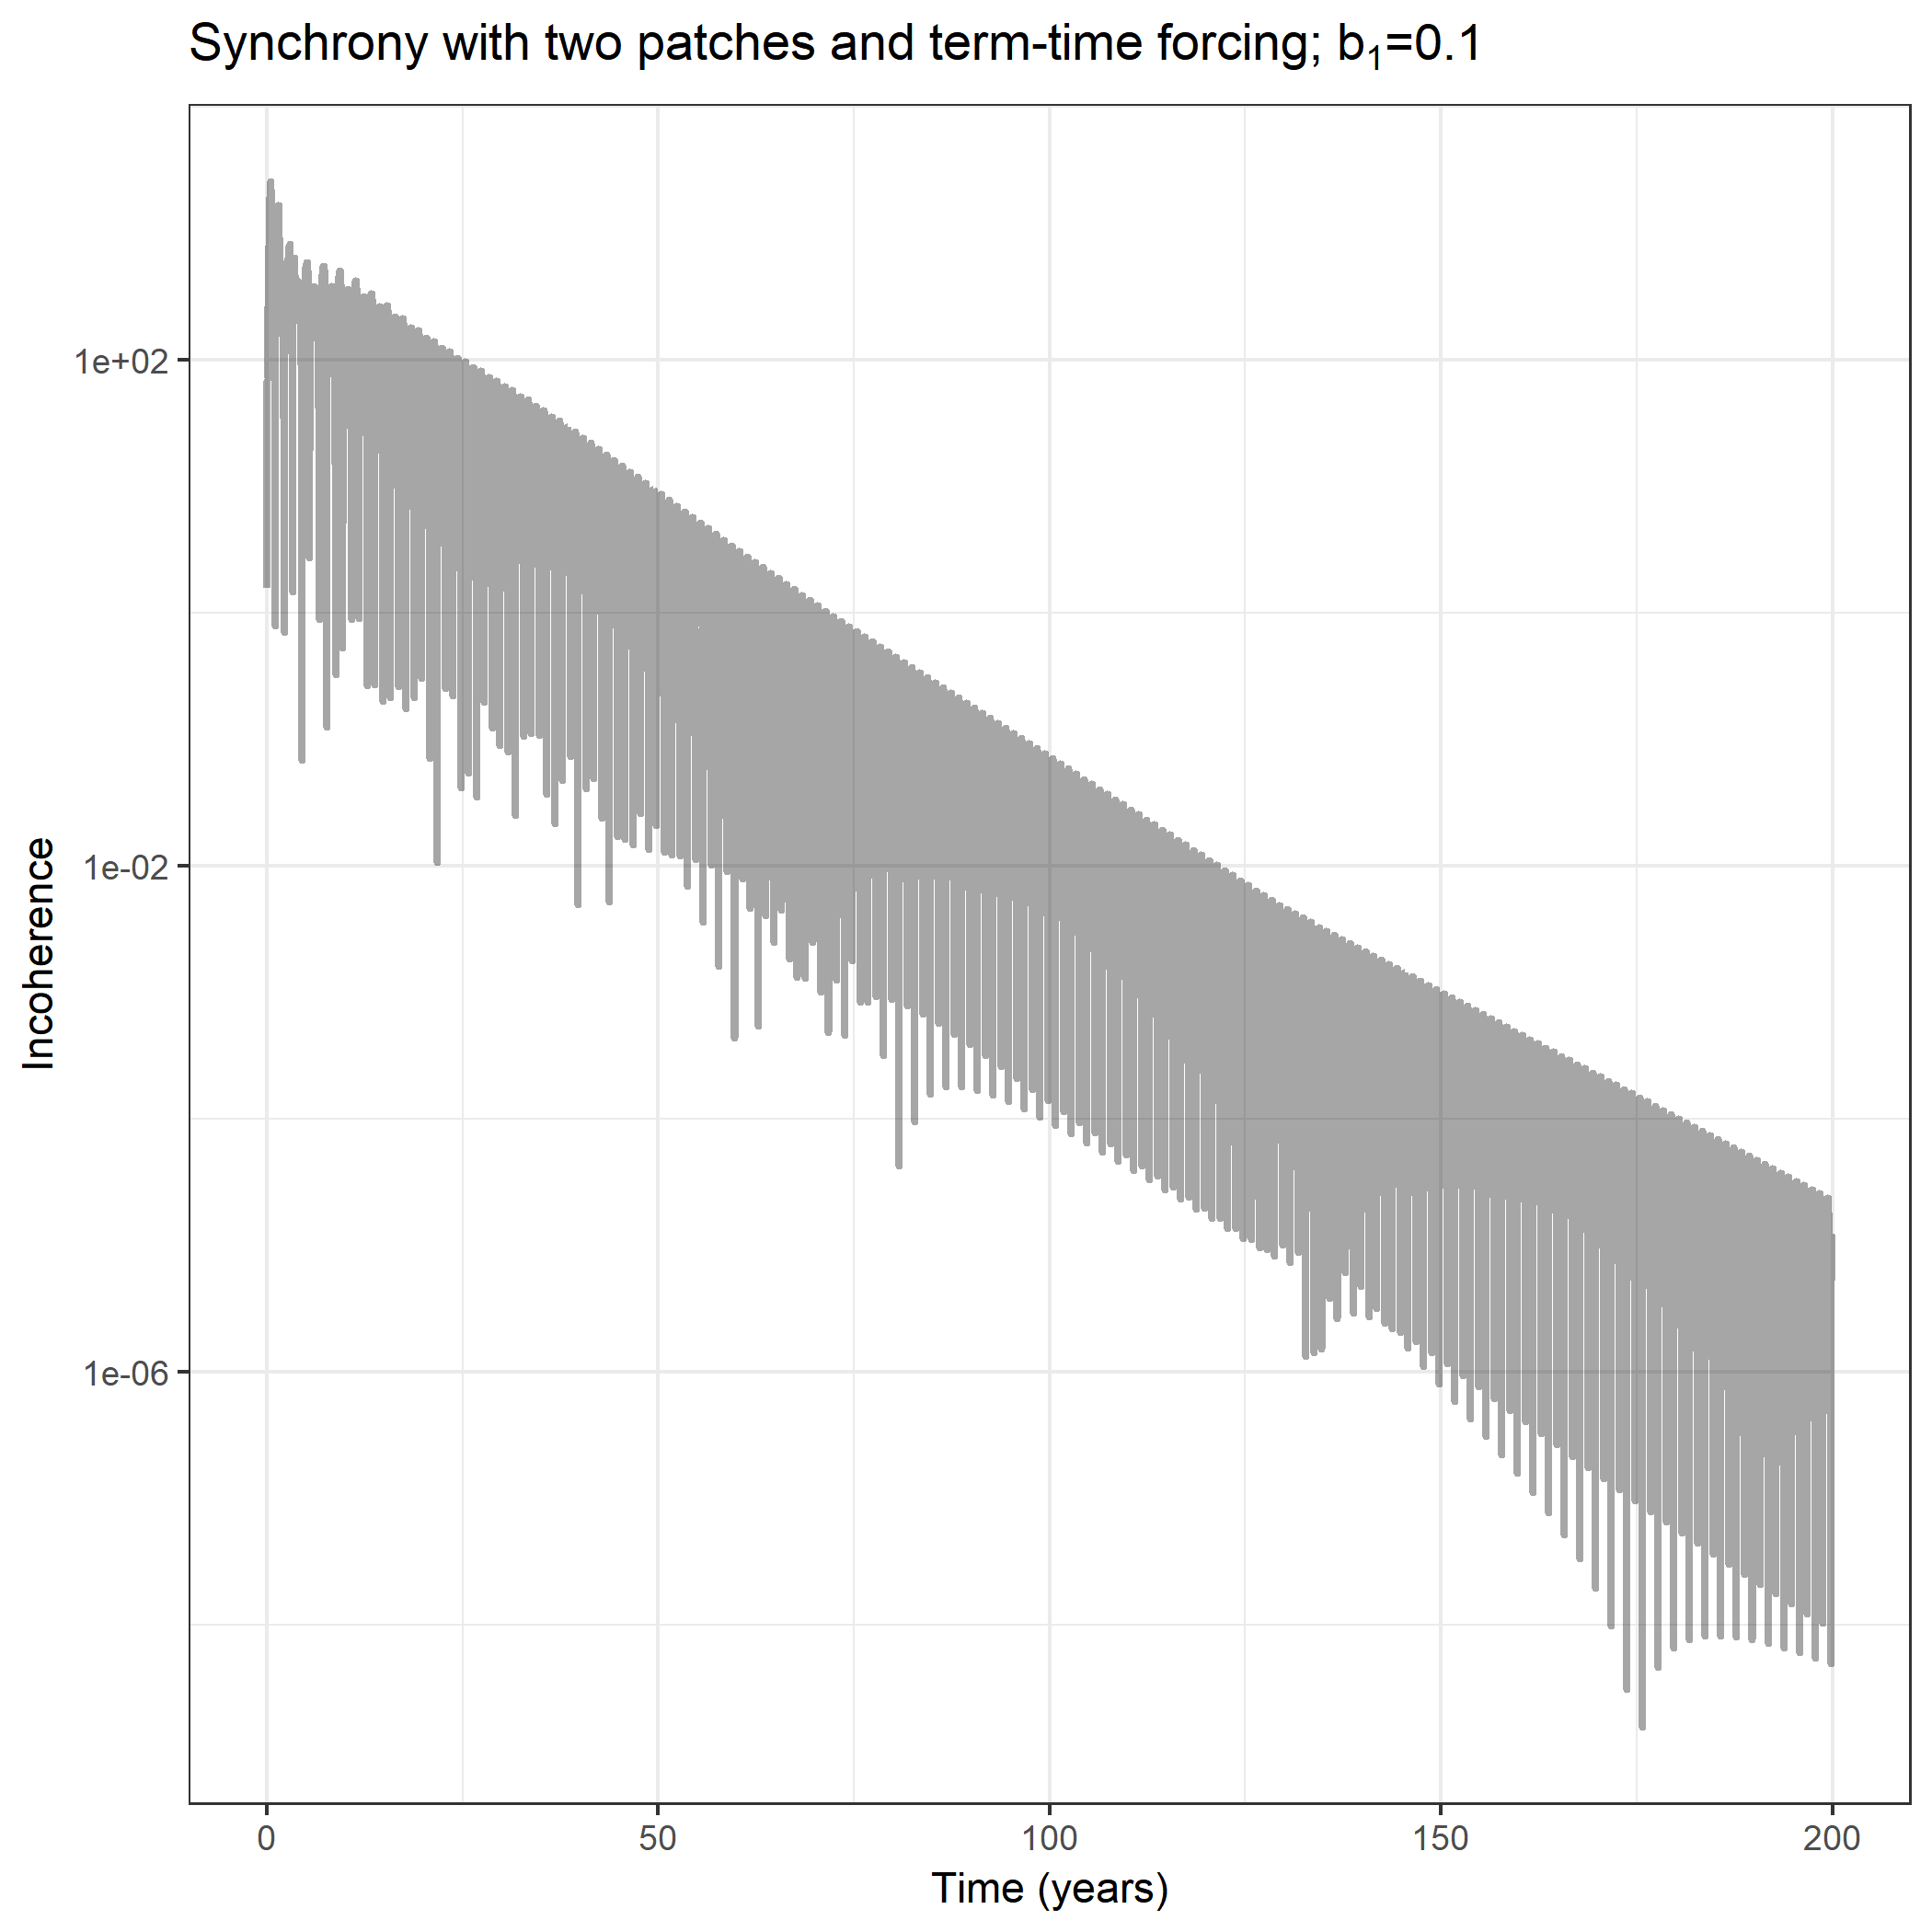
\includegraphics[width=.4\linewidth]{seasonalamp_3.png}} \quad
\subfloat{(d)}
{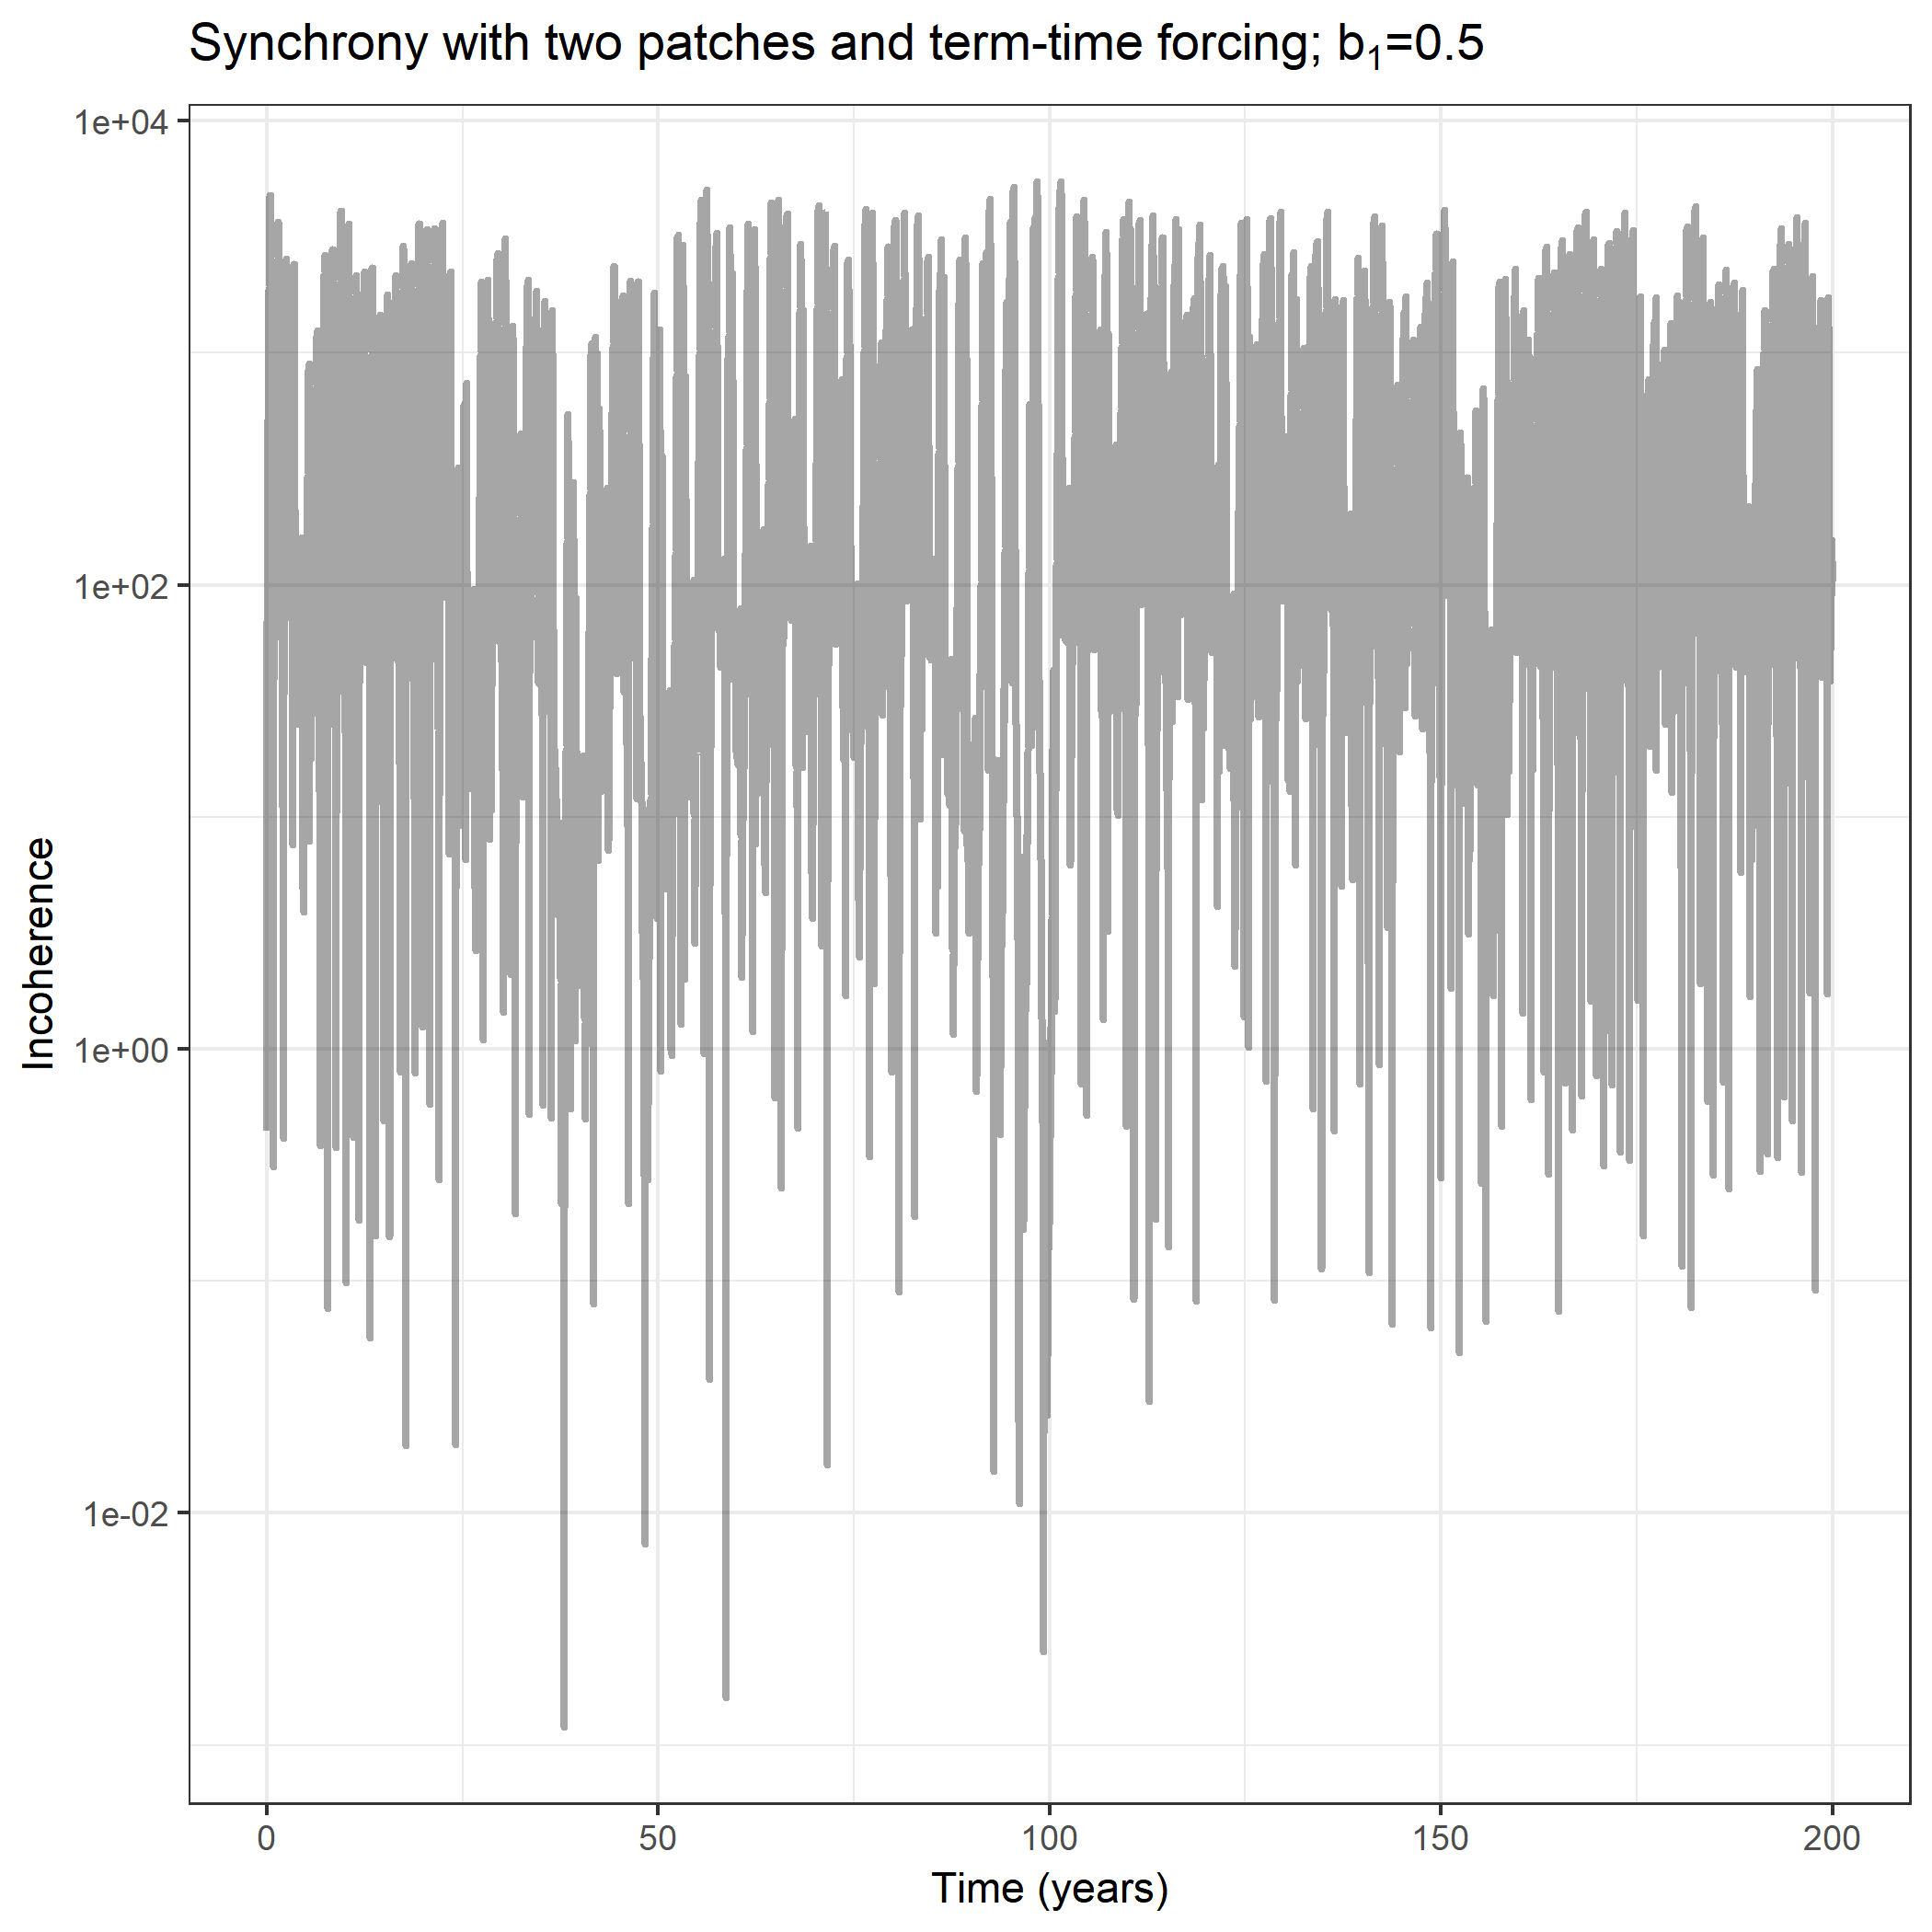
\includegraphics[width=.4\linewidth]{seasonalamp_4.png}} \\
\caption{Synchrony in two equally mixing patches, with sinusoidally forced transmission rate ((a) and (b)), and term-time forced transmission rate ((c) and (d)). Furthermore, the seasonal amplitude is also varied; (a) and (c) have a seasonal amplitude of 0.1, while (b) and (d) have a seasonal amplitude of 0.5. The initial population sizes are $N_1=N_2=10^6$, and all initial conditions are retrieved from \cite{earn1998persistence}. \label{fig:seasamp}}
\end{figure}

We observe \autoref{fig:seasamp}, which plots the log of incoherence against time. We notice that when a sinusoidally-forced transmission rate is used, coherence does not occur at all when the seasonal amplitude is equal to 0.1, and very little coherence occurs as the seasonal amplitude is raised to 0.5. Furthermore, no simple trend in coherence is detected either. This is to say that an increase in seasonal amplitude does not necessarily coincide with an increase in coherence, which in turn leads us to suspect that the bifurcation diagram with respect to the seasonal amplitude $b_1$ has chaotic regions interspersed with ``sensible regions" (regions containing 1-cycles and 2-cycles, for example).

When observing the effects of the term-time forced transmission rate, we discover that the opposite results occur. At a seasonal amplitude of $b_1 = 0.1$, coherence is observed, but at a seasonal amplitude of $b_1 = 0.5$, no coherence is observed. Regardless of the transmission function used, we can conclude that the existence of synchrony between patches depends on the seasonal amplitude $b_1$, and that a more thorough investigation of the effects of $b_1$ on coherence is required. 
Some future goals of this project, as they pertain to the effects of seasonal amplitude, include:

\begin{enumerate}

\item Create a bifurcation diagram ($b_1$ on the x-axis, prevalence on the y-axis) to determine the existence of chaotic regions and "sensible regions". This will help in determining which seasonal amplitudes result in synchrony between patches.

\item Determine the likelihood of synchrony, i.e. ``synchrony impossible'', ``synchrony possible'', ``synchrony inevitable''.

\item Create a measure of synchrony to better understand the potential differences in degrees of synchrony.

\item Iterate through random sets of initial conditions to observe if the effects of seasonal amplitude change depending on the initial conditions.

\end{enumerate}

\subsection{Mixing Structure}
\label{ss:mixingstructure}
Here we will investigate coherence under different connectivity structures. We vary the connectivity matrix $M$ with all the other parameters at base values. We begin by first looking at the 2-patch case.

In the equal coupling regime, the connectivity matrix $M$ is given by
\begin{equation}
\begin{bmatrix}
p &		{1-p} \\
{1-p} &		p
\end{bmatrix},
\end{equation}
where we can interpret $p$ as the proportion of individuals that interact only within their own patch. 

We performed numerical simulations using $p = 0, 0.25, 0.5, 0.75, 0.999$, with 20 random initial conditions at each $p$. Interestingly, preliminary numerical results (as seen in \autoref{fig:mix}) show that for all choices of $p$ most initial conditions result in synchrony. However, there seem to be some rare initial conditions for which the system does not synchronize.

\begin{figure}
\centering
\subfloat
{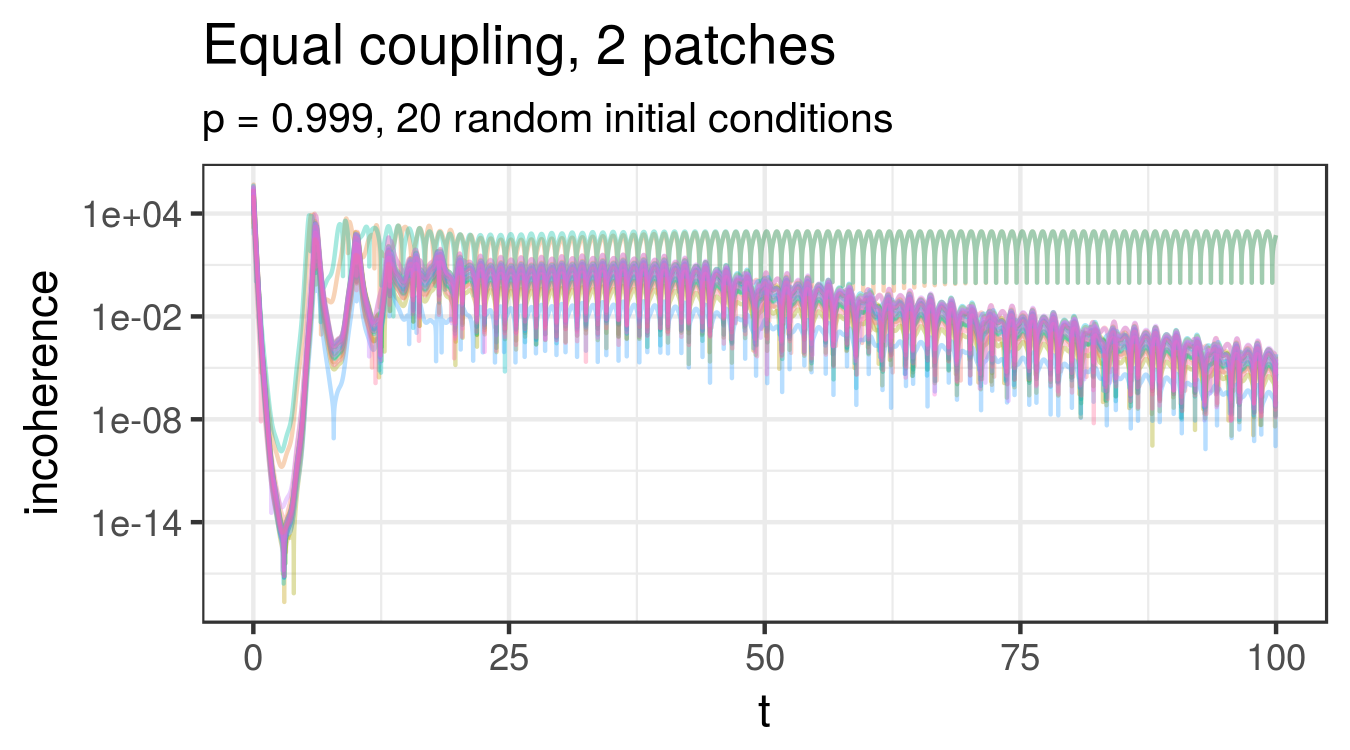
\includegraphics[width=.6\linewidth]{mixfig/eq99.png}} \\
\subfloat
{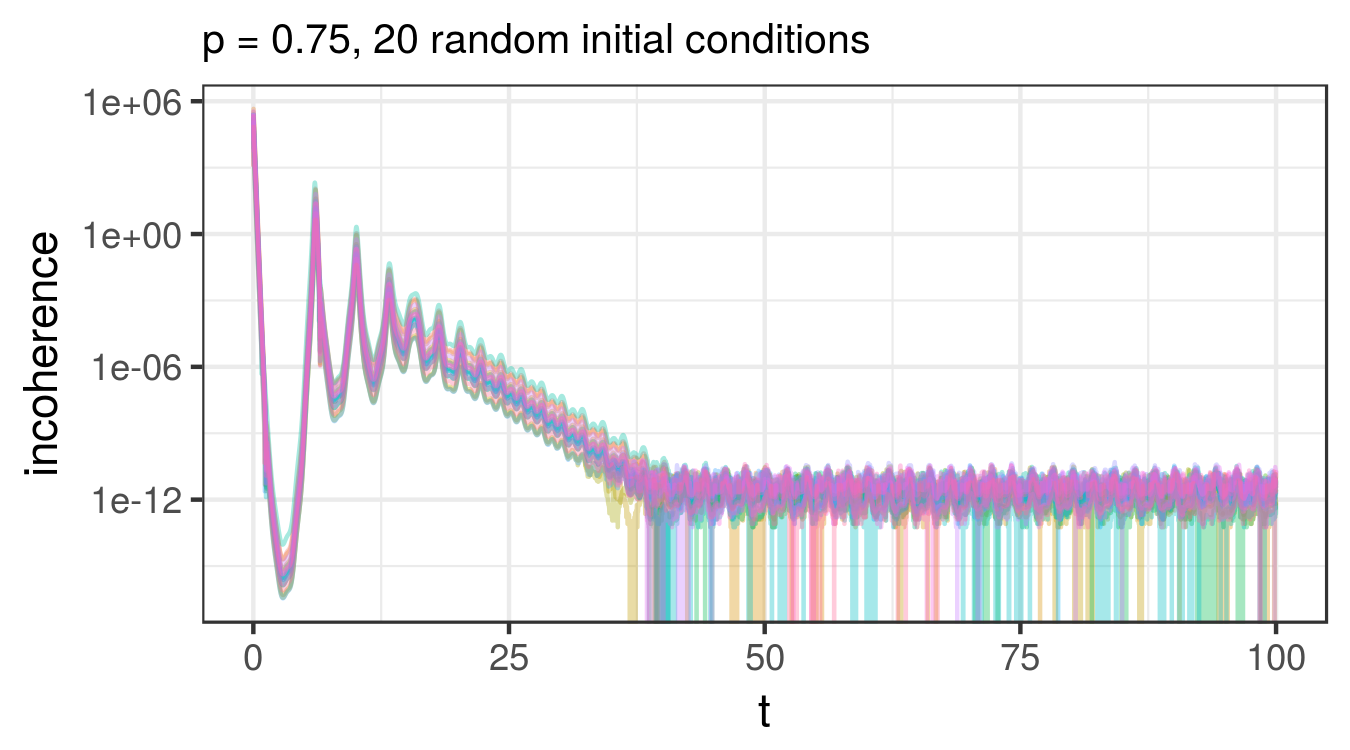
\includegraphics[width=.45\linewidth]{mixfig/eq75.png}} \quad
\subfloat
{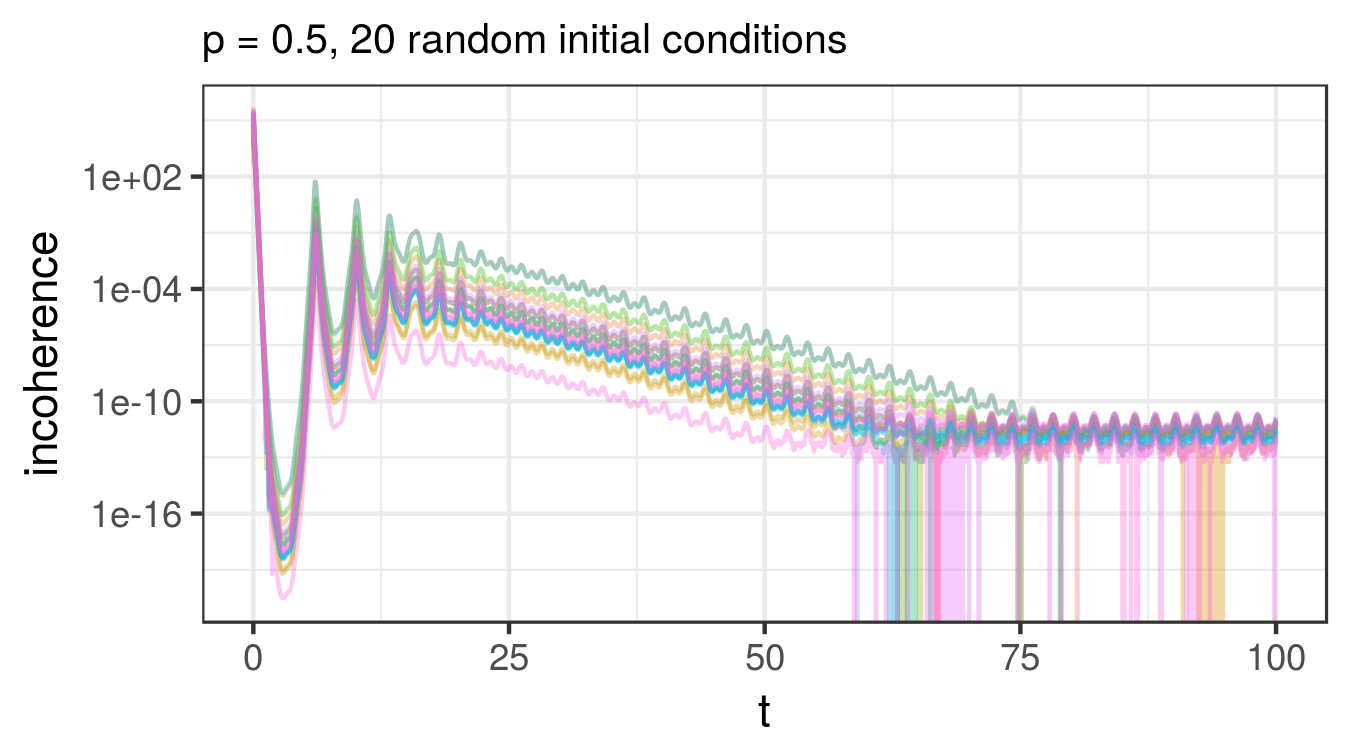
\includegraphics[width=.45\linewidth]{mixfig/eq50.png}} \\
\subfloat
{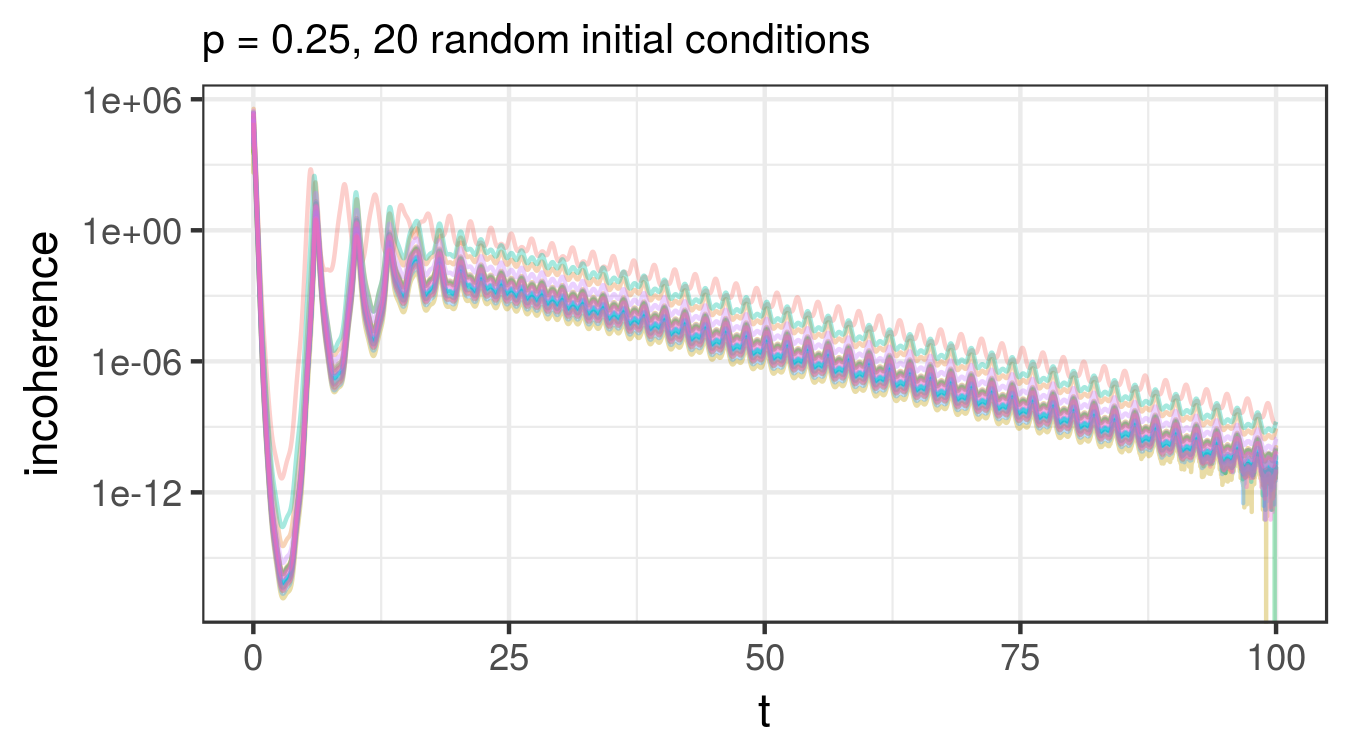
\includegraphics[width=.45\linewidth]{mixfig/eq25.png}} \quad
\subfloat
{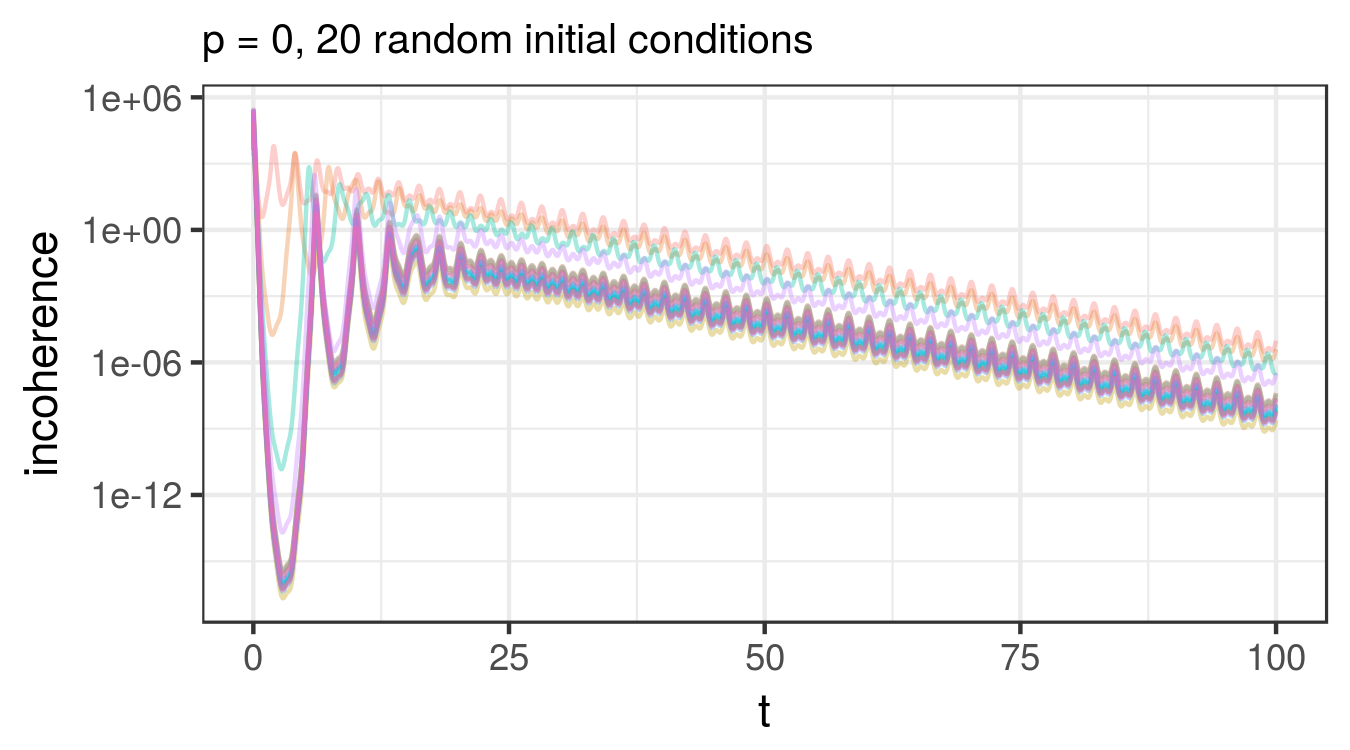
\includegraphics[width=.45\linewidth]{mixfig/eq0.png}} \\
\caption{Synchrony in two equally mixing patches, varying the proportions $p$ that interact only in their own patch. There exist initial conditions in the $p = 0.999$ case where the patches do not synchronize.} \label{fig:mix}
\end{figure}

With these initial results in mind, we have several goals in this section for the final report.
\begin{enumerate}
\item We observe that we have exponential decay of incoherence for the patches that do synchronize, and furthermore the rate increases with $p$ up to $p = 0.75$. We wish to see how this decay rate changes with $p$.
\item Construct a measure of synchrony. For instance, we might take the maximum incoherence measure in the last 10 years of the simulation, or take the decay rate.
\item Search the $p$ parameter space with higher resolution and more initial conditions (in particular for the $p = 0.999$ case) so that we can better understand which initial conditions result in asynchrony.
\item Investigate other connectivity matrices. Since individuals are not moving between patches, we may relax the condition on the column and row sums adding to 1.
\item If time allows, explore cases with $m > 2$ patches.
\end{enumerate}



\subsection{Parameter Space}
\label{ss:parameters}
We now examine the effects of changing $\R_0$ on synchrony. For our initial investigations, we will follow the values for the connectivity matrix and the initial conditions supplied in \cite{earn1998persistence}. When preliminary numerical experiments with these parameters are performed, it becomes apparent that whether (or not) we get synchrony between patches has a dependency on the $\R_0$ parameter. An illustrative example of this is shown in \autoref{fig:coherencetwopatchesR0}. This figure, which plots the log of incoherence against time, shows that the $\R_0=12$ case appears to approaching synchrony while the $\R_0=17$ case does not.  
\begin{figure}
\centering
\subfloat[$\R_0=17$]
{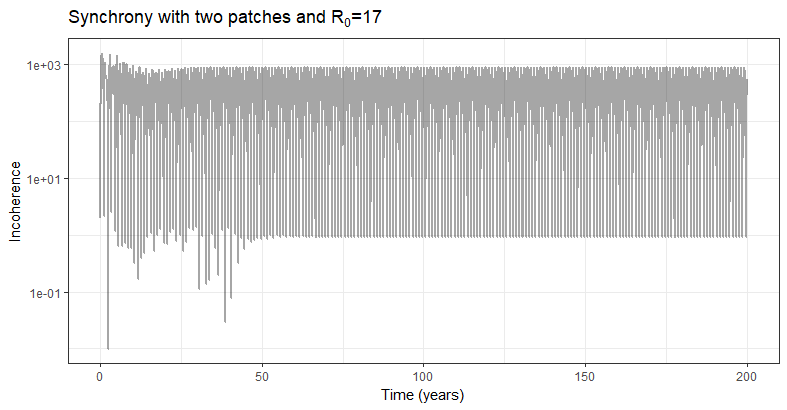
\includegraphics[width=.65\linewidth]{R017Coherence}} \\ \quad
\subfloat[$\R_0=12$]
{\label{fig:example-b}
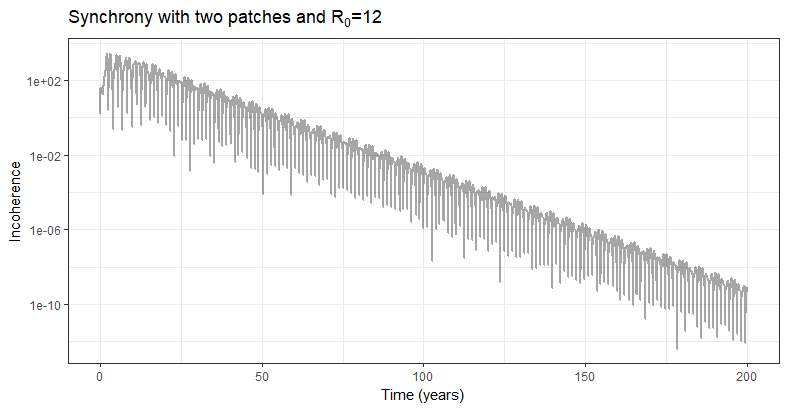
\includegraphics[width=.65\linewidth]{R012Coherence}} \\
\caption[Tu duo titulo debitas latente]{A run of a two patch model with initial population of $N_1=N_2=10^6$. The initial conditions (following \cite{earn1998persistence}) were $S_1=0.05N_1$, $I_1=0.0001N_1$, $S_2=0.07N_2$, $I_2=0.0001N_2$.  The connectivity matrix was $\begin{bmatrix}
0.999 & 0.001\\
0.001 & 0.999
\end{bmatrix}$. The plots show the results when running for 200 years with a time step of 1 day.} \label{fig:coherencetwopatchesR0}
\end{figure}

This initial result indicates that a more thorough investigation of coherence when changing $\R_0$ is needed. Thus, (for the final paper) we will next produce a bifurcation diagram (based on a single patch) with $\R_0$ on the x-axis and prevalence on the y-axis. We will additionally mark on this diagram the proportion of runs (with different initial conditions) in which a two patch system demonstrates synchrony at those $\R_0$ and prevalence values. This numerical exploration of synchrony will be used to quantify how likely synchrony is with those parameters. This diagram will be similar to Figure 1 in \cite{Earn2000conservation}, but our numerical experiments with synchrony will take the place of the analytically identified regions of `synchrony impossible', `synchrony possible', and `synchrony inevitable'. 

\subsection{Stochasticity}
\label{ss:stochasticity}

Note that coherence cannot occur once we allow for demographic stochasticity. For this draft, we outline two main ideas that we want to explore in this section.
Throughout this section, we use the following dispersal matrix:
$$
\begin{bmatrix}
0.999 & 0.001\\
0.001 & 0.999
\end{bmatrix}
$$

The first idea is to explore how stochasticity changes synchrony between patches. In \autoref{fig:stoch1}, we observe that the system changes from synchrony to asynchrony and goes back to synchronyous state again. We would like to quantify a degree of synchrony and how much of it is affected by stochasticity.

\begin{figure}
\centering
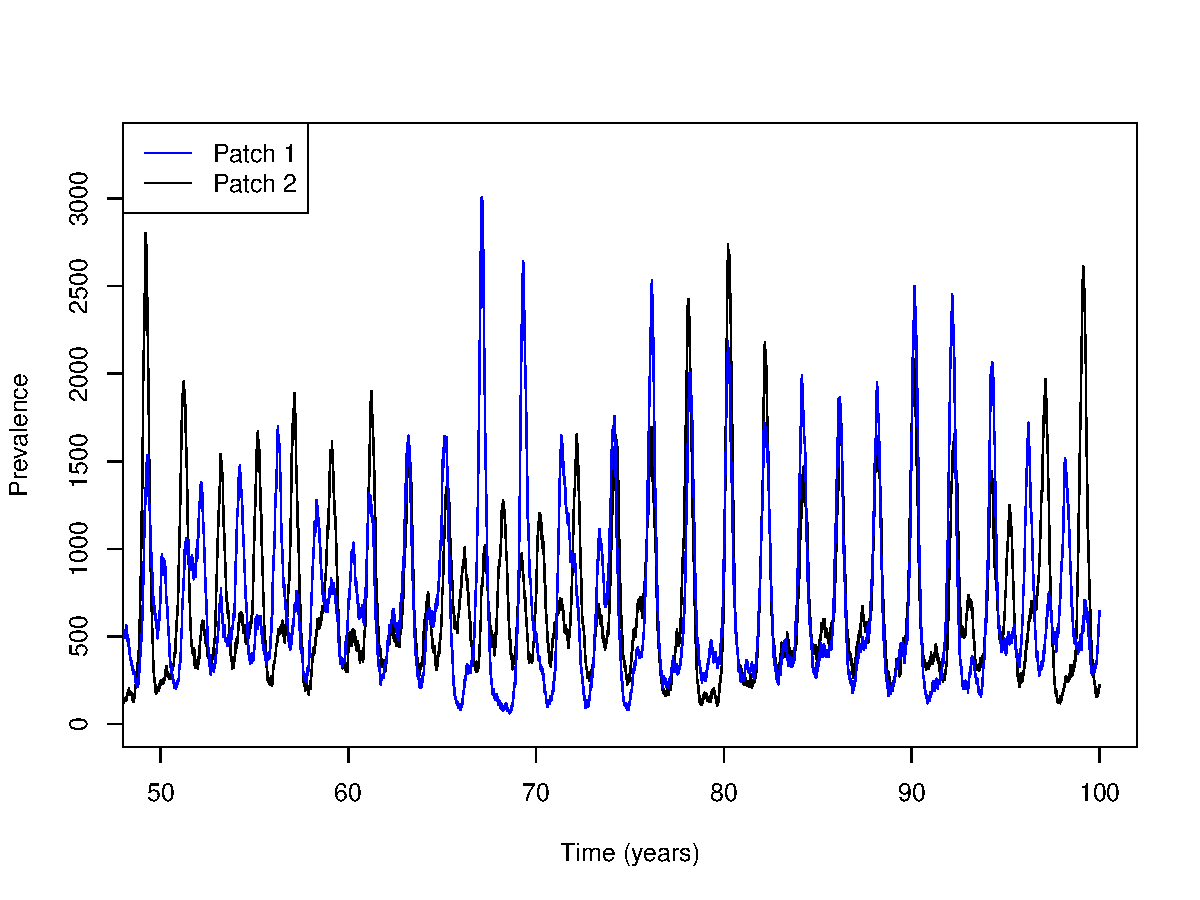
\includegraphics[width=.65\linewidth]{stochfig/stochastic1.pdf} 
\caption[???]{Here is the caption}\label{fig:stoch1}
\end{figure}

The second idea is to explore idea of the ``rescue effect''. In \autoref{fig:stoch1}, we reduced the population size in each to 70\% to allow for stochastic drift in the population. Here, we observe that even when there is very little dispersal among patches, a patch that is at its peak can save other patches and allow epidemic to begin again. Without dispersion, patches that suffer from random drift will no longer suffer from outbreaks.

\begin{figure}
\centering
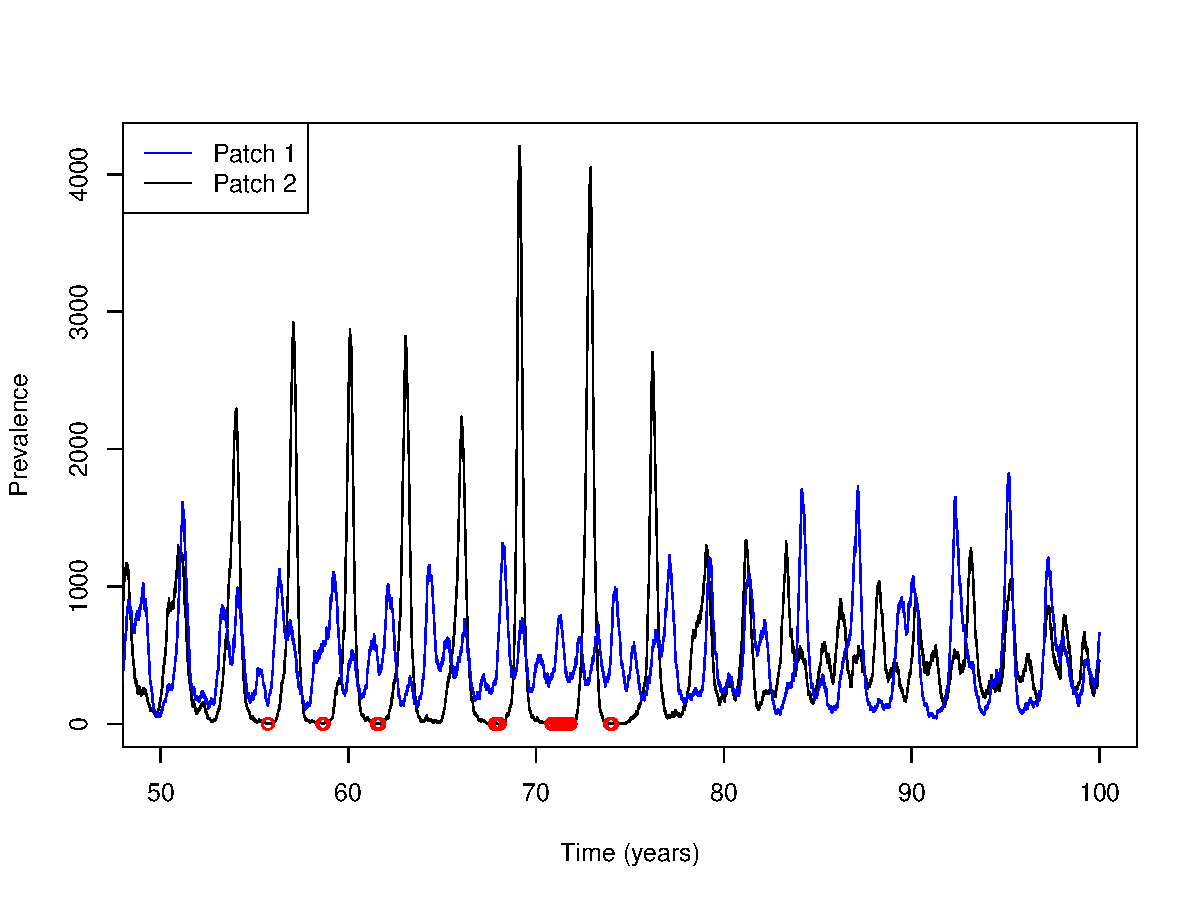
\includegraphics[width=.65\linewidth]{stochfig/stochastic2.pdf} 
\caption[???]{Red represents time step in which number of infected individuals in patch 2 is equal to zero.}\label{fig:stoch2}
\end{figure}


\section{Discussion}
\label{sec:discussion}

\bibliographystyle{vancouver}
\bibliography{synchrony}
\end{document}